\begin{figure}[H]
    \centering
    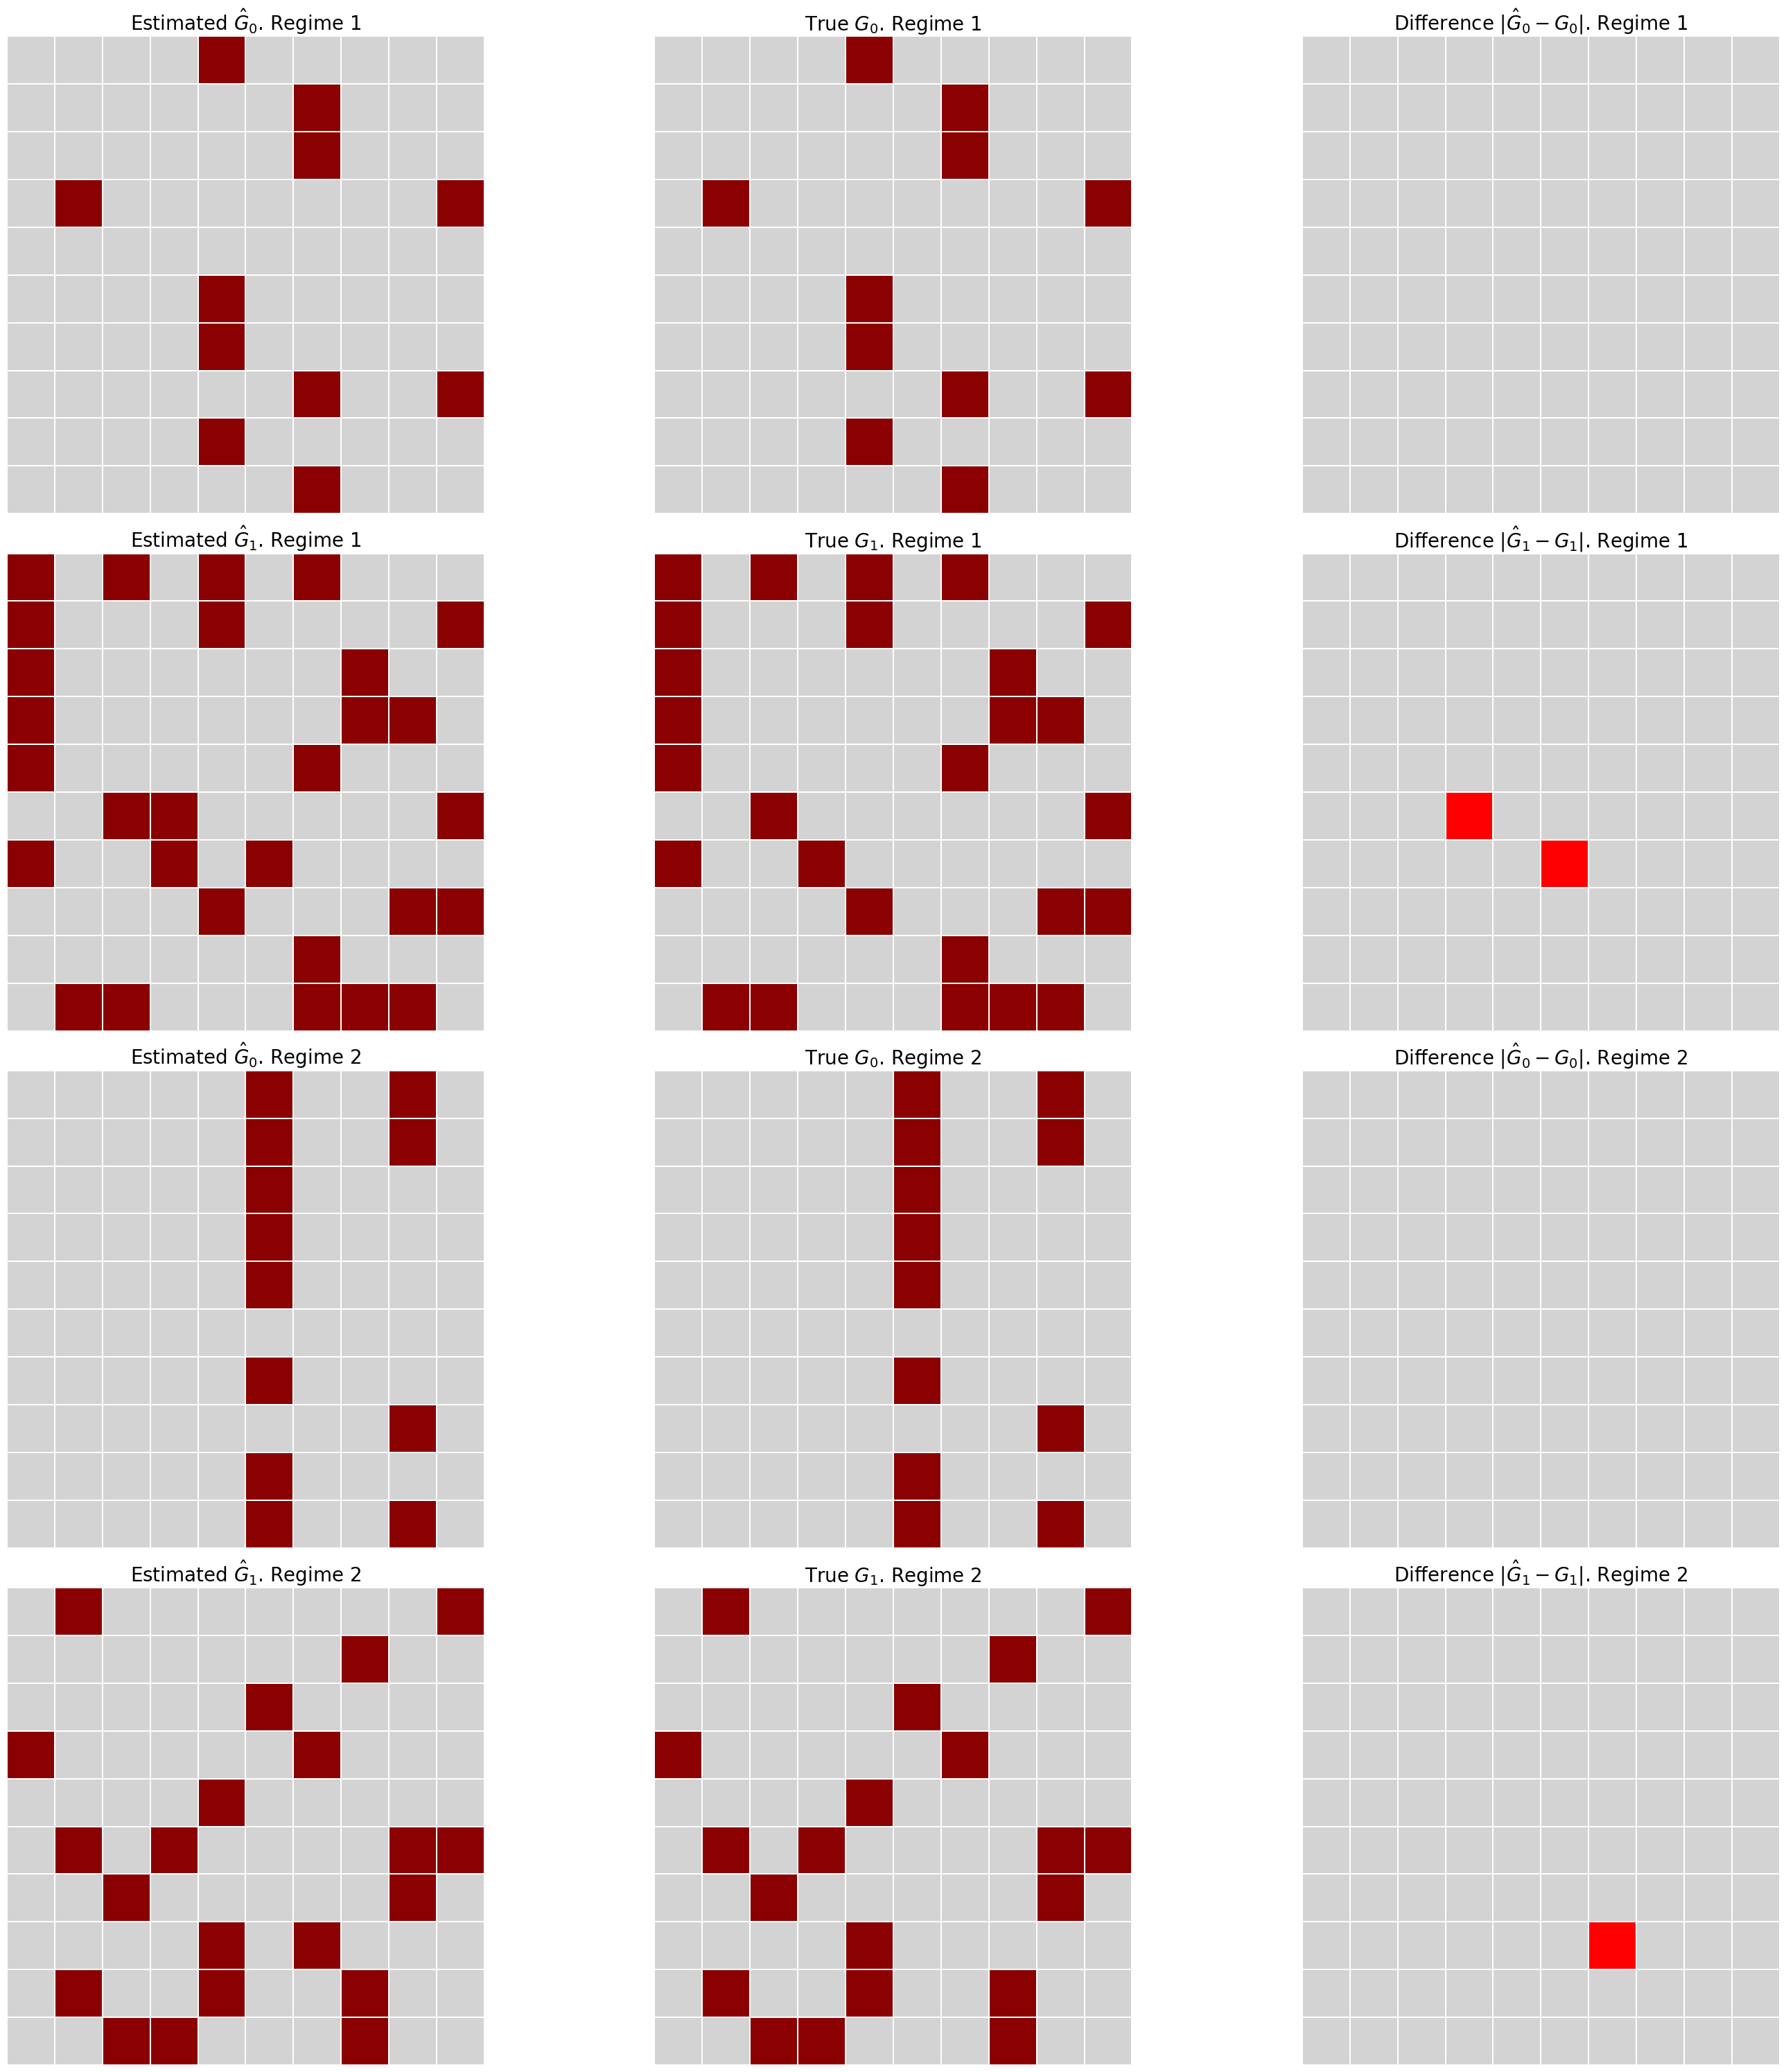
\includegraphics[width=1\linewidth]{figures/10nodes_2reg.png}
    \caption{The estimated temporal causal graphs for two regimes, in \textcolor{teal}{Heteroscedastic case}, consist of one matrix of 10 rows and 10 columns representing instantaneous links and another of 10 rows and 10 columns delineating time-lagged relations (with a maximum lag $L=1$ in this case). Dark red indicates a value of one (presence of an edge), while gray symbolizes a value of 0 (absence of an edge). The second column displays the ground-truth causal graphs, and the final column highlights the difference between the estimated and true graphs.}
    \label{fig:enter-label}
\end{figure}

\begin{figure}[H]
    \centering
    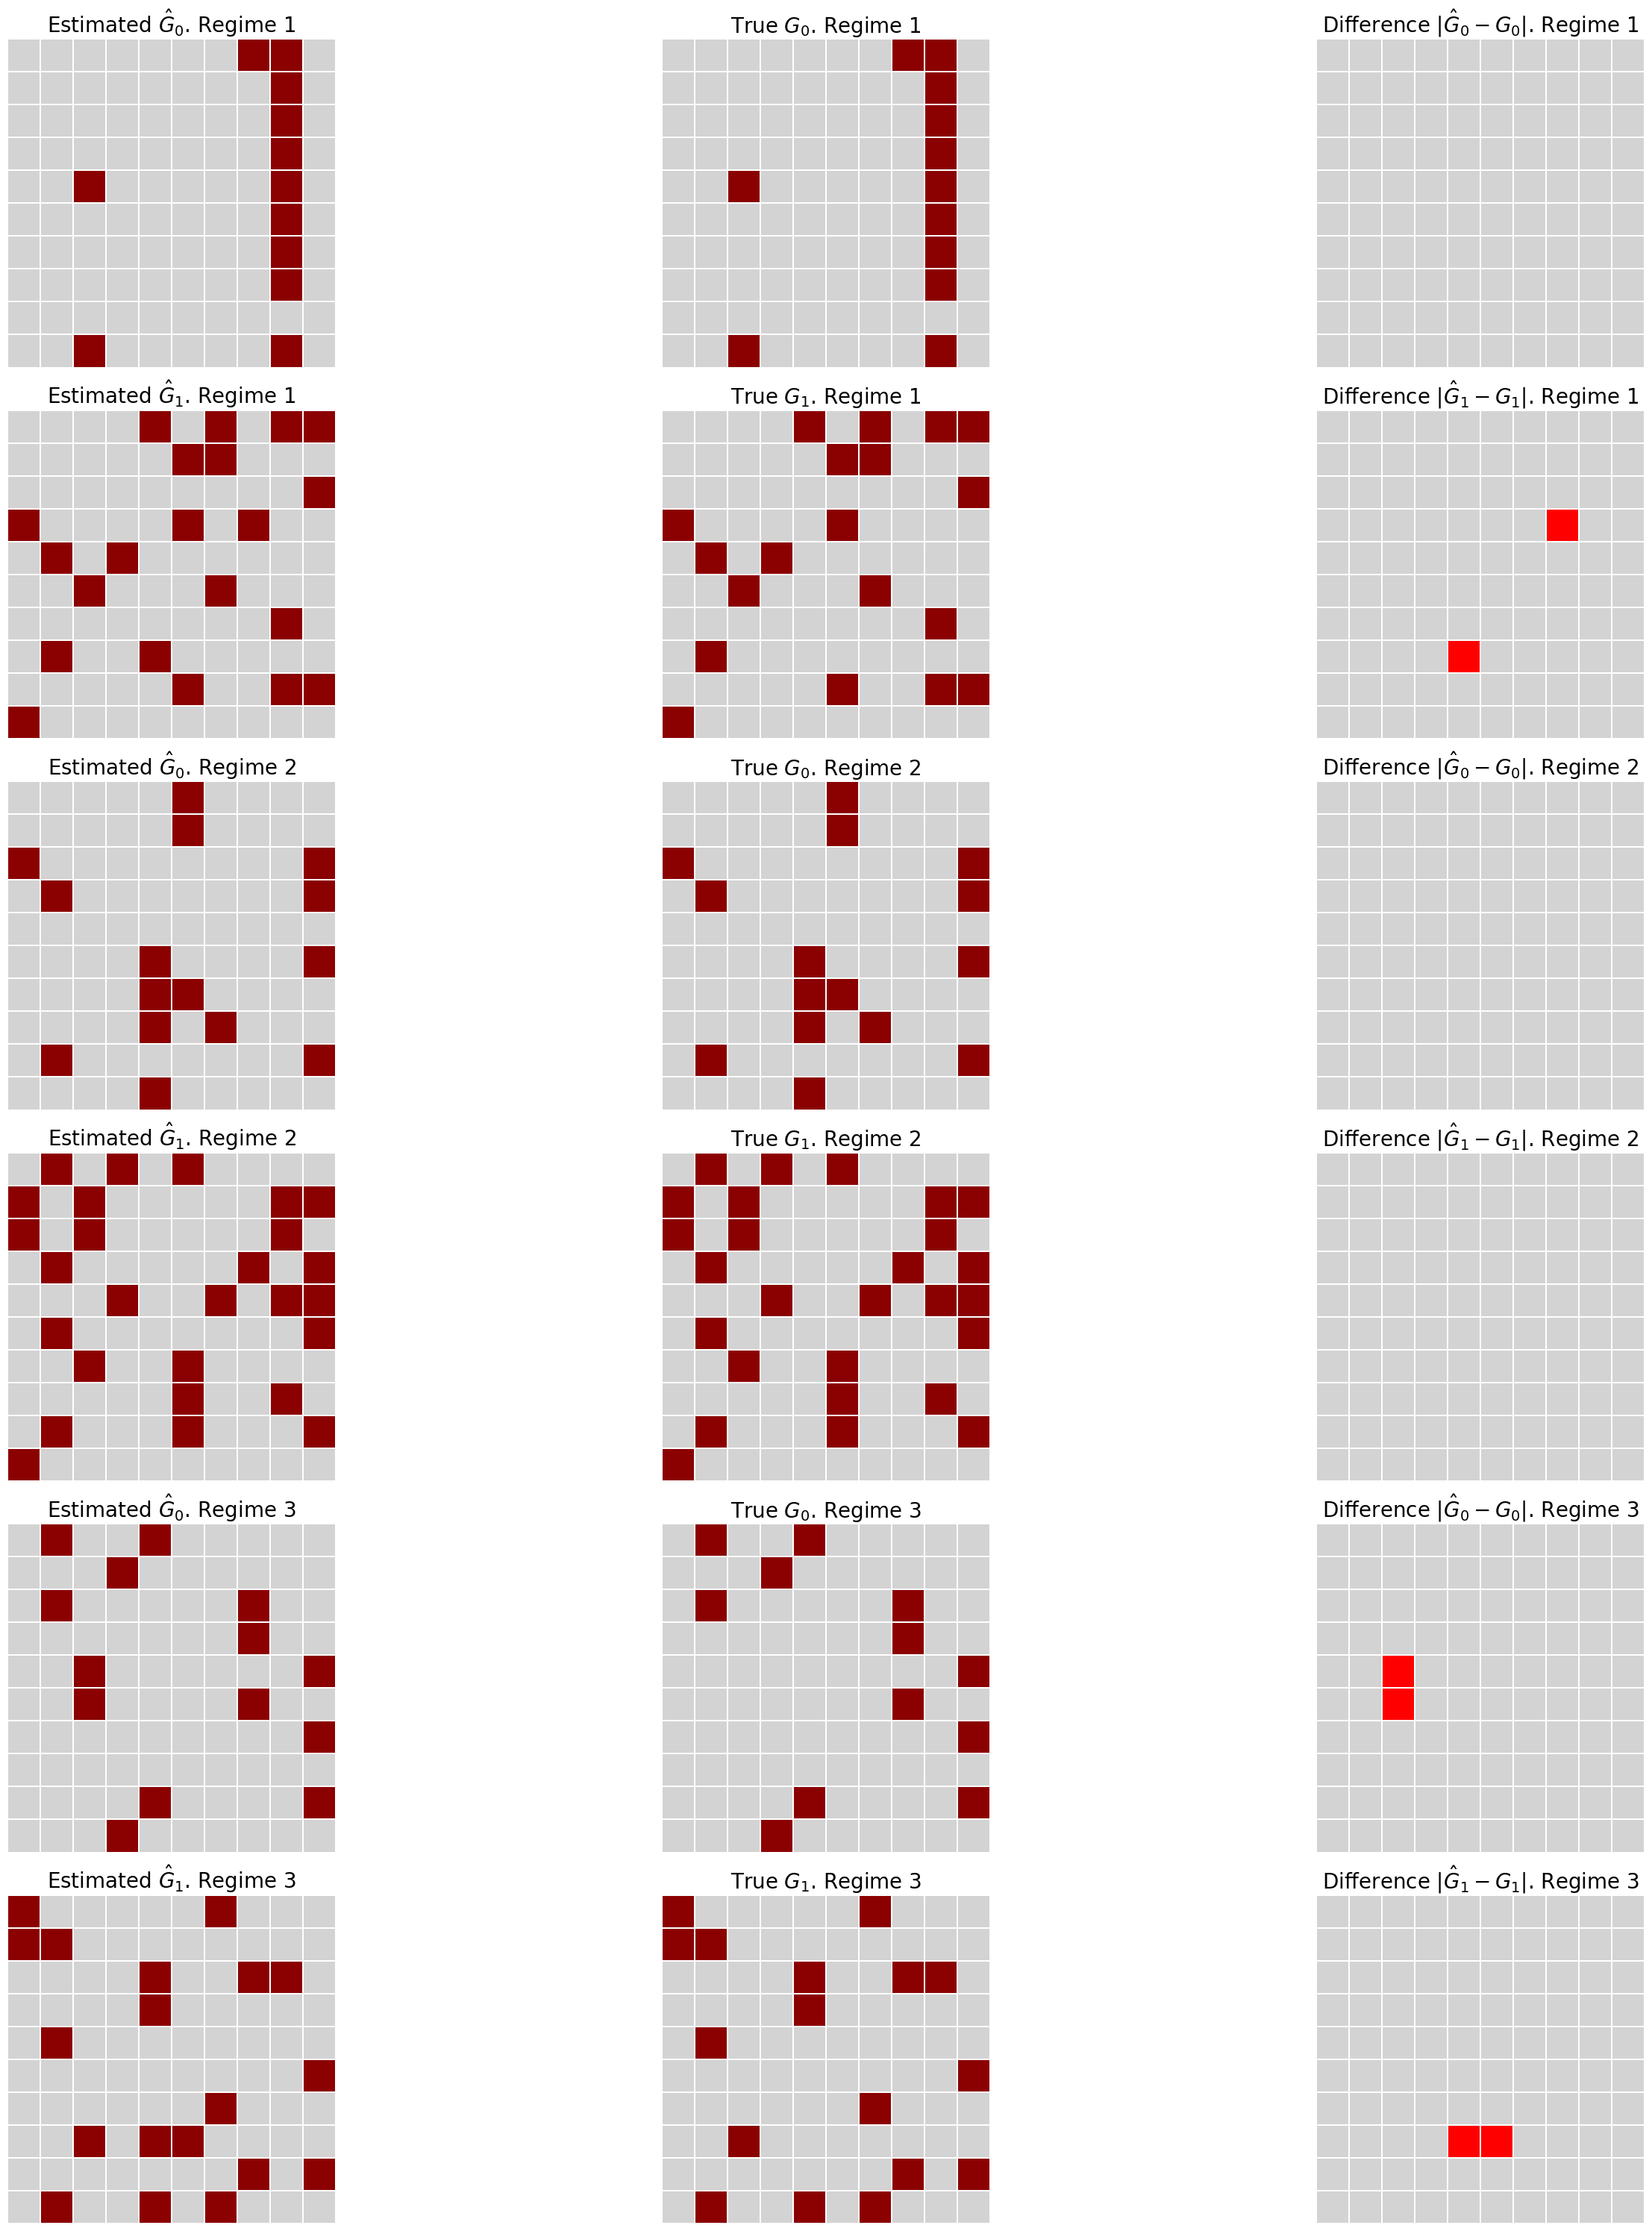
\includegraphics[width=0.9\linewidth]{figures/10nodes_3reg_exp3.png}
    \caption{The estimated temporal causal graphs for three regimes, in \textcolor{teal}{Heteroscedastic case}, consist of one matrix of 10 rows and 10 columns representing instantaneous links and another of 10 rows and 10 columns delineating time-lagged relations (with a maximum lag $L=1$ in this case). Dark red indicates a value of one (presence of an edge), while gray symbolizes a value of 0 (absence of an edge). The second column displays the ground-truth causal graphs, and the final column highlights the difference between the estimated and true graphs.}
    \label{fig:enter-label}
\end{figure}

\begin{figure}[H]
    \centering
    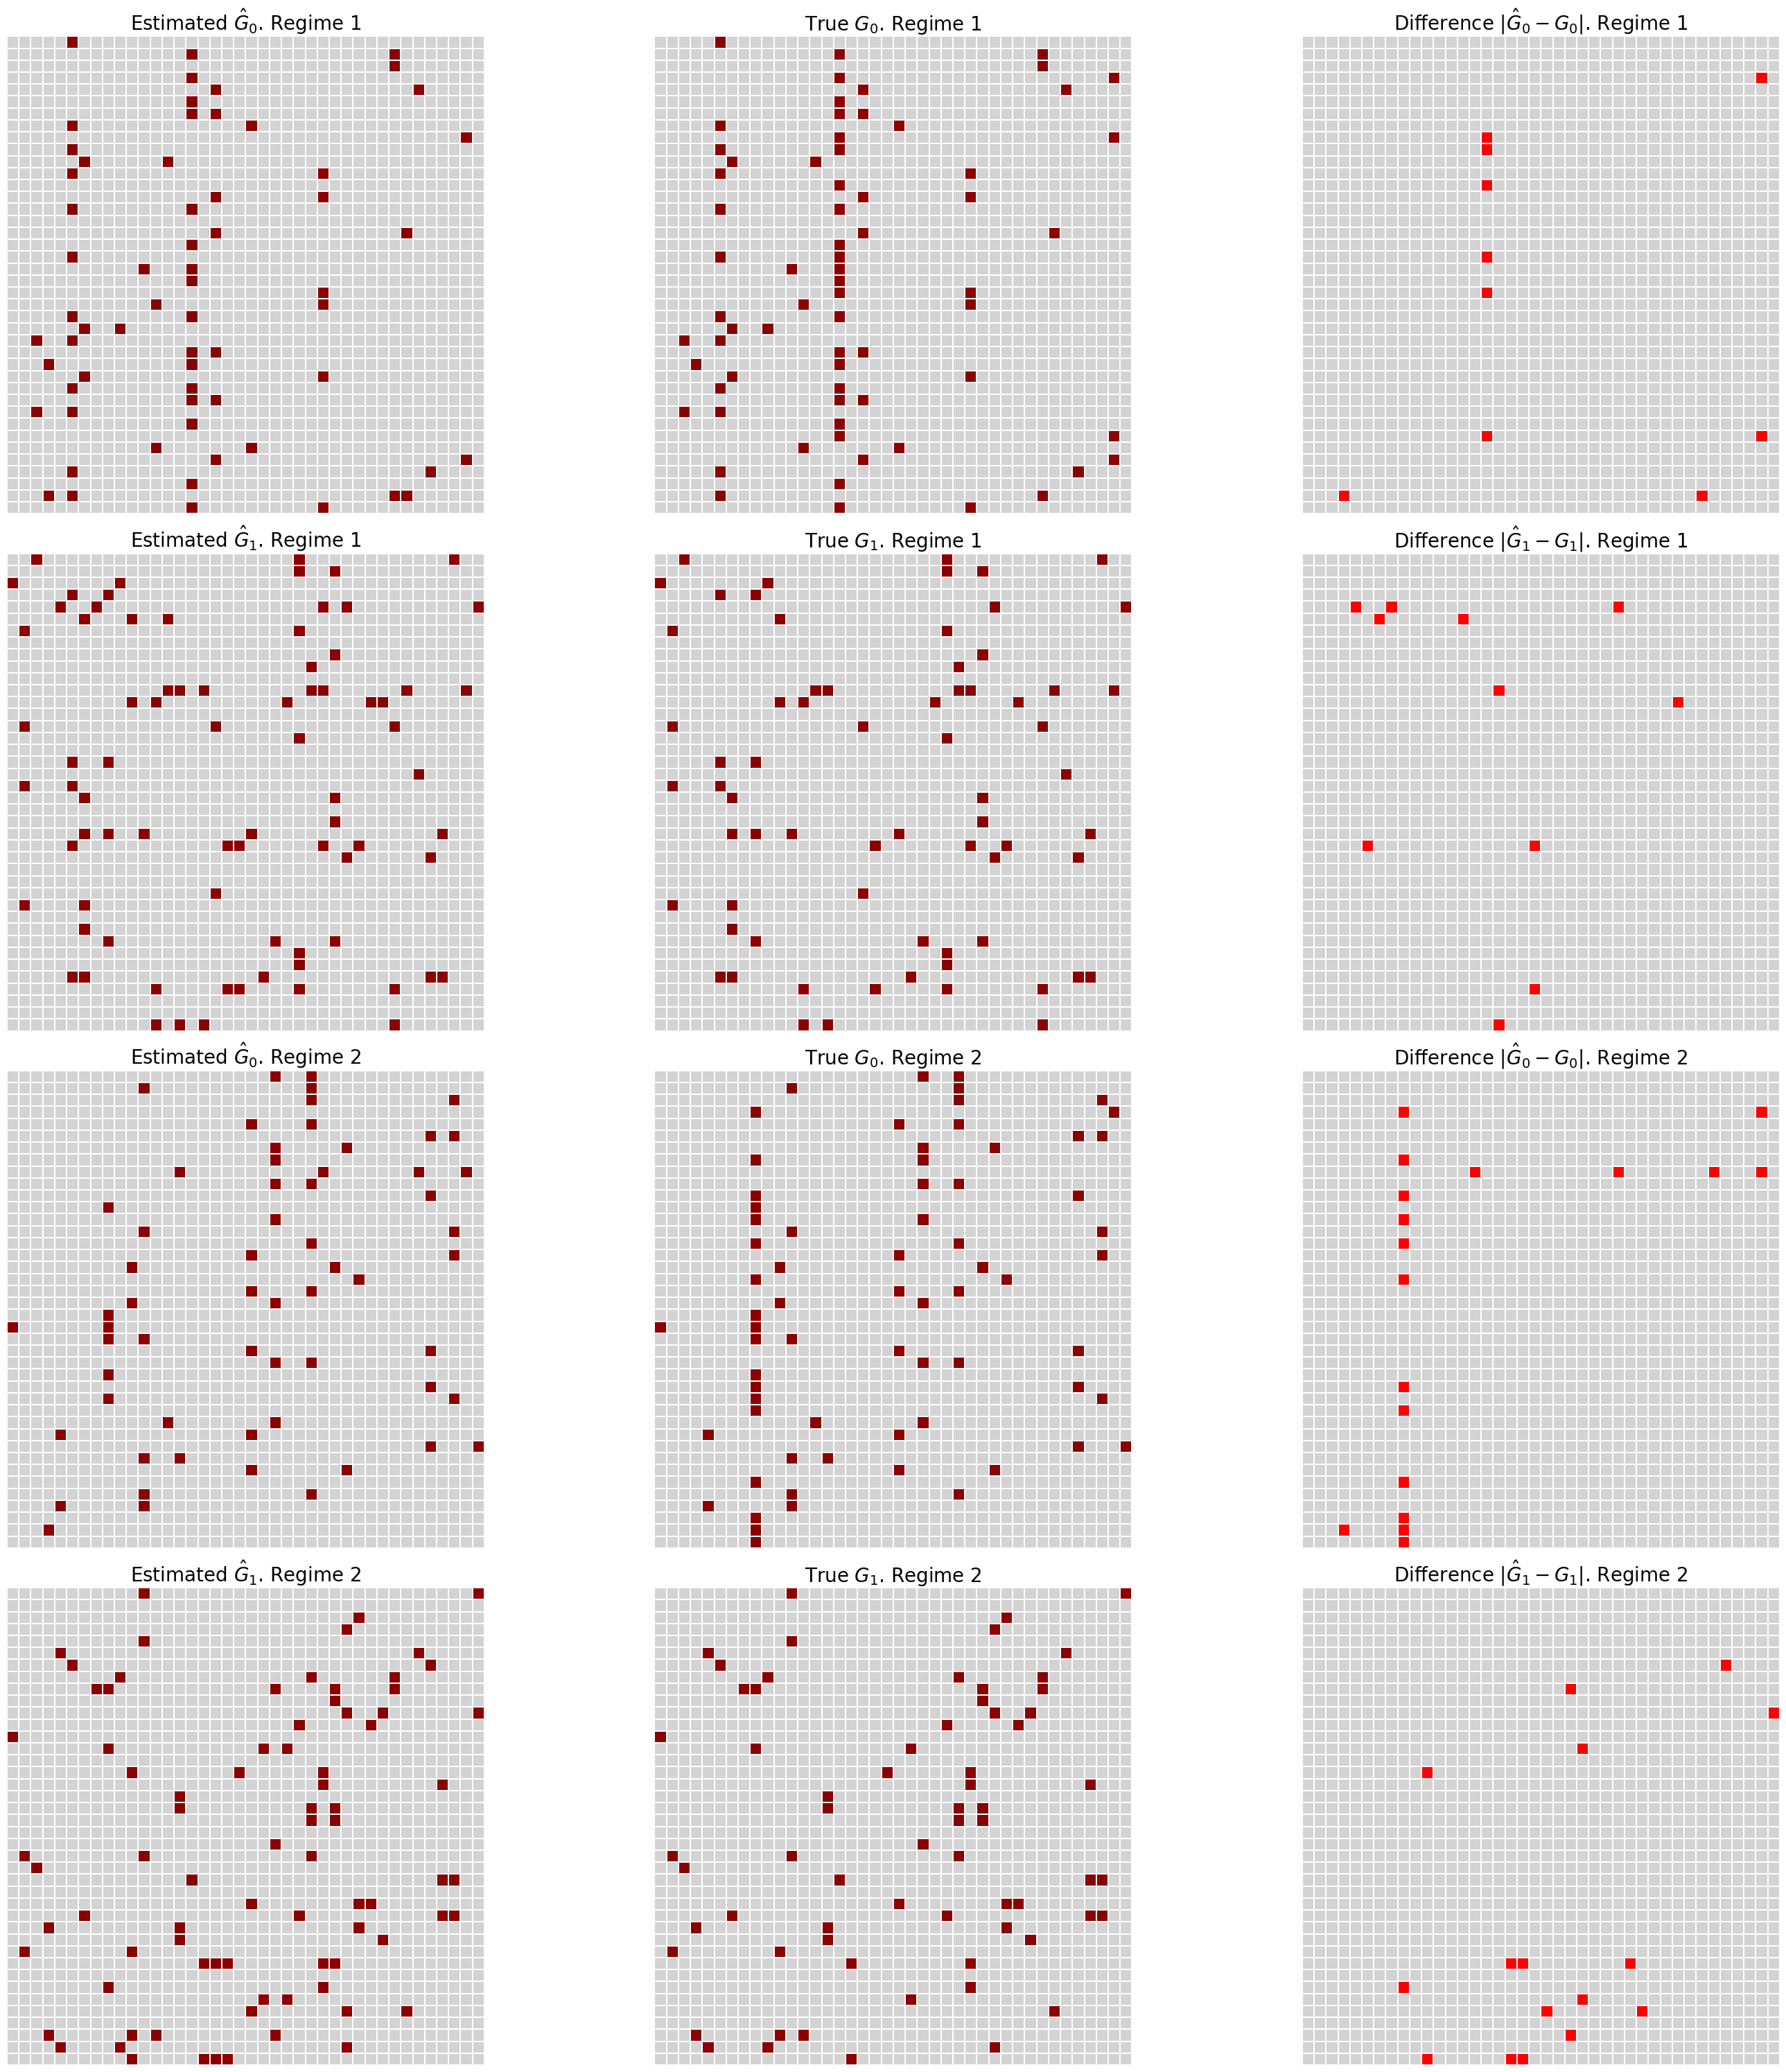
\includegraphics[width=1\linewidth]{figures/40nodes_2reg_2exp.png}
    \caption{The estimated temporal causal graphs for three regimes, in \textcolor{teal}{Heteroscedastic case}, consist of one matrix of 40 rows and 40 columns representing instantaneous links and another of 40 rows and 40 columns delineating time-lagged relations (with a maximum lag $L=1$ in this case). Dark red indicates a value of one (presence of an edge), while gray symbolizes a value of 0 (absence of an edge). The second column displays the ground-truth causal graphs, and the final column highlights the difference between the estimated and true graphs.}
    \label{fig:enter-label}
\end{figure}
\begin{figure}[H]
    \centering
    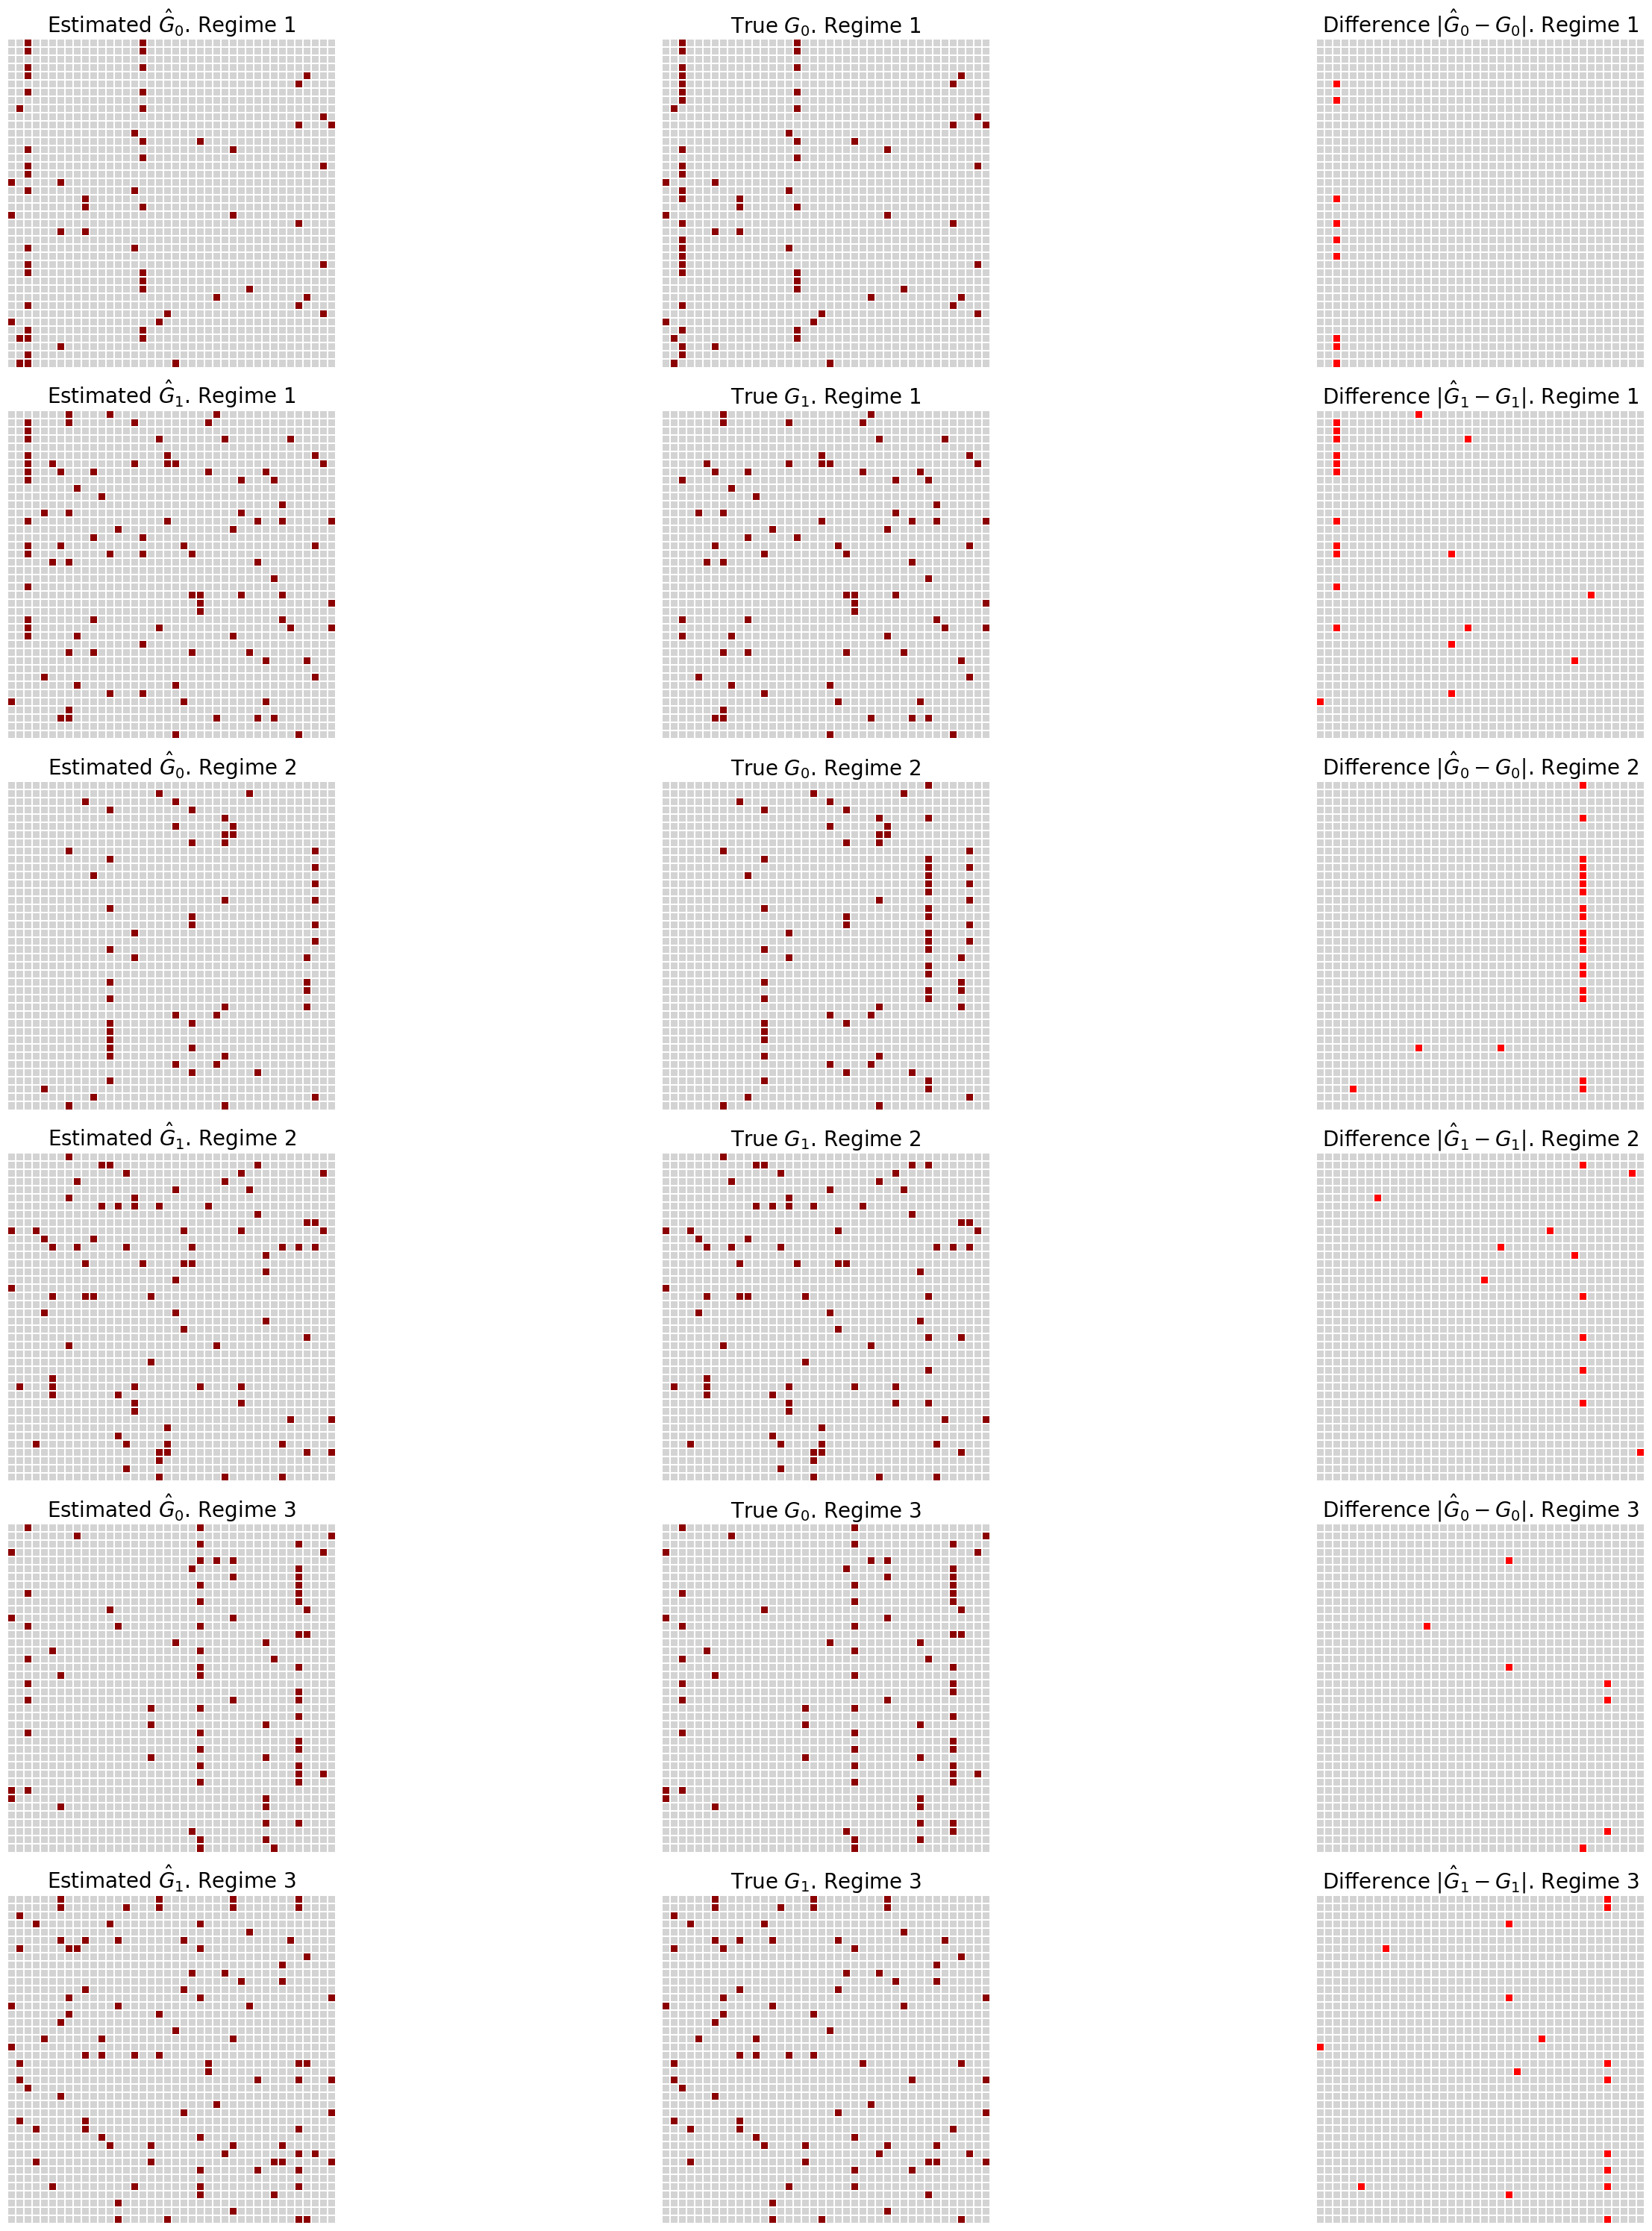
\includegraphics[width=0.9\linewidth]{figures/40_3reg_non_gauss.png}
    \caption{The estimated temporal causal graphs for three regimes, in \textcolor{teal}{Non-Gaussian case}, consist of one matrix of 40 rows and 40 columns representing instantaneous links and another of 40 rows and 40 columns delineating time-lagged relations (with a maximum lag $L=1$ in this case). Dark red indicates a value of one (presence of an edge), while gray symbolizes a value of 0 (absence of an edge). The second column displays the ground-truth causal graphs, and the final column highlights the difference between the estimated and true graphs.}
    \label{fig:enter-label}
\end{figure}